\documentclass{article}

\usepackage{listings}
\usepackage{graphicx}
\usepackage{fullpage}
\title{MADden}
\author{Morgan Bauer 9890-4838 \\
         Christan Grant 8143-3970 \\
         Joir-dan Gumbs 6148-9357}
\date{2011-09-22}
\begin{document}
	\maketitle
	\section{What are we doing?}
	We plan to provide a web-based interface for interacting with
	sports data.
	\subsection{What are \textbf{the} data sources?}
	The data we are using is scraped ESPN NFL data, NFL related 
	tweets, team blogs, etc. The scraped ESPN NFL data contains the
	play-by-play info for every NFL game, player statistics, team
	statistics, and division blogs.
	\subsection{The data product}
	Visualizations of:
	\begin{enumerate}
		\item[1] Correlations between game actions, such as:
		\begin{enumerate}
			\item[A] Outcome of coin toss for home/away team
			\item[B] Probability of making field goal based on
			         stadium (by distance of attempt)
			\item[C] Fan sentiment with game outcome.
		\end{enumerate}
		\item[2] Summary of team performance
		\item[3] Tweet density for every game
		\item[4] ... and other things yet to be discovered
	\end{enumerate}
	\subsection{What is the piece of framework we aim to build?}
	An extensible, interactive, query-driven framework for sports
	intelligence. We can run complex queries over heterogeneous data.
	For example:
		Given a set of Games $G$ where $G.hometeam$ and $G.awayteam$.
		and  a set of tweets $T$ where 
			for $t \in T$, 
				we can extract: 
					sentiment information $s(t)$ and teamnames $teamnames(t)$.
 
		
\lstset{frame=single }
\lstset{basicstyle=\footnotesize}
\begin{lstlisting}[language=SQL]
SELECT hometeam, AVG(s(t))
FROM T, G
WHERE hometeam = teamnames(t)
GROUP BY hometeam
\end{lstlisting}

This result of the this query is a list of the home team sentiment for
a selection of games. We could also set a range for the time in the tweet.
Notice we had perform both sentiment analysis, information extraction (finding
team names) and a poor mans entity-resolution in resolving the team names.
This is an example of the type of queries we which to support.

\begin{figure}
	\begin{center}
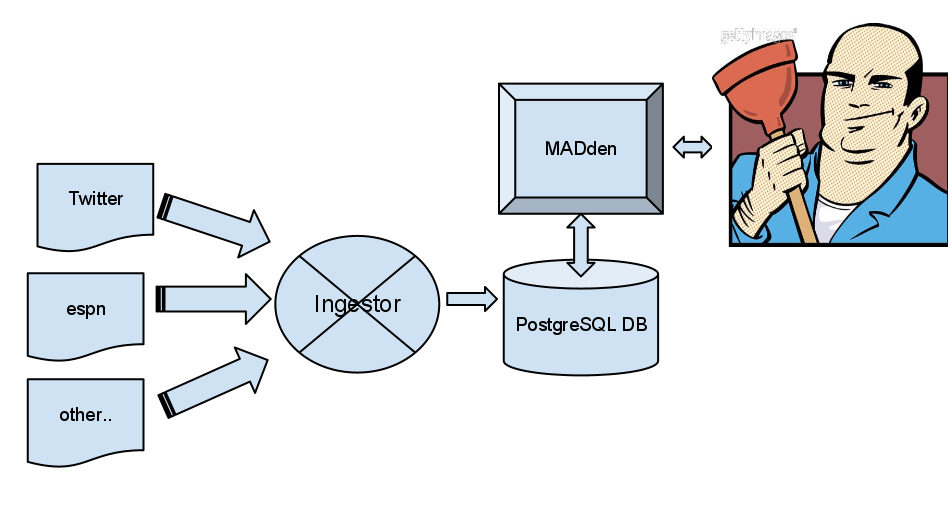
\includegraphics[width=104mm]{architecture-1.png}
\caption{System Architecture}
\label{fig:architecture}
\end{center}
\end{figure}


The \ref{fig:architecture} describes the architecture of our product.
We have an Ingestors that pull structured data in from different sources.
The ingestor is generic and can be created to adapt to different type of 
data. The MADden interface takes queries performs client-side logic to all
the user to view the results of their queries.

	\section{What is related work and state-of-the-art}
	NFL.com, ESPN.com, Yahoo Sports all do sports statistics. 
	Polaris, IBM ManyEyes, Tableau all have done visualization tools.
	MADLib is what we are basing our project on.
	\section{Why is it an important project for Data Science?}
	We are using all tools of data science. Scraping dirty data and turning
	it into clean information, and then presenting the information in an easy
	to digest form.
	\section{What are the novelties of the project? What is the end goal?}
	A system that allows for tinkering with sports data for gaining insight 
	of team/player performance and fan sentiment.
	\section{What is the measure of success?}
	When we are able to perform queries for one user correlating the
	different datasets, and it "makes sense."
	 
\end{document}
